%%%%%%%%%%%%%%%%%%%%%%%%%%%%%% -*- Mode: Latex -*- %%%%%%%%%%%%%%%%%%%%%%%%%%%%
%%% al_intro.tex --- 
%%% Author          : blehr
%%% Created On      : Thu Mar 18 04:05:10 1993
%%% Last Modified By: blehr
%%% Last Modified On: Sun Apr 11 13:59:32 1993
%%% RCS revision    : $Revision: 1.10 $ $Locker:  $
%%% Status          : In writing....
%%%%%%%%%%%%%%%%%%%%%%%%%%%%%%%%%%%%%%%%%%%%%%%%%%%%%%%%%%%%%%%%%%%%%%%%%%%%%%

\section{Introduction}
\label{algo:intro}

In this chapter, the proposed eye-tracking algorithm is given a
thorough presentation.  The name of the algorithm, {\octopus}, arises
from the fact that the search part of the algorithm can be compared to
a four-armed octopus looking for the sea.  Also, the line-oriented
edge detection, as described in the previous chapter, is for each
iteration performed in a pattern similar to an eight-armed octopus.

\subsection{Problem Definition and Clarification}
\label{algo:intro:problem}

The problem definition to which my thesis work has been related was
given as the {\em algorithmic\/} problem definition in
Section~\ref{intro:problem}.  For the sake of easy reference, it is
repeated here:

\paragraph{Problem definition:}
Design, implement and, as extensively as possible, test an algorithm
to, on the basis of a given image of the eye, determine the position
of the (centre of the) pupil, relative to some given reference point.
The algorithm must to be fast enough to run in the CPU of the
computer, and has to satisfy the following requirements:
\begin{itemize}
\item The position of the pupil is to be determined with an accuracy
  corresponding to 1 pixel in the digitized image.
\item Whenever the pupil cannot be found (due to blinking,
  disturbances, etc.), an error signal is to be given.
\item The total running time of the algorithm may not exceed 20 ms in
  the worst case.
\end{itemize}
Whether the accuracy requirement above complies with
requirement~\ref{req:2} in Section~\ref{intro:motivation} depends on
the resolution of the image and on the fraction of the image occupied
by the pupil.  Preferably, the image should have a resolution of
$512\times 512$ pixels with 256 gray levels, and the eye should fill
the entire image.
\vspace*{0.5cm}

\noindent Some vague points in this definition have to be clarified
before continuing the presentation of the algorithm.  These are:
\begin{description}
\item[Reference point:] ``{\em\ldots determine the position\ldots
    relative to some reference point\ldots\/}'' The upper left corner
  of the image has been used as reference point, having coordinates
  $(0,0)$.
\item[Error signal:] ``{\em\ldots an error signal is to be
    returned\ldots\/}'' The procedure implementing Step 1 of the basic
  algorithm formulation given in Section~\ref{eval:approach:algo} has
  been implemented as a boolean function, returning {\em false\/} if
  a pupil point cannot be found in an image.
\item[Resolution:] ``{\em Preferably, the image should have a
    resolution of 512$\times$512 pixels with 256 gray levels, and the
    eye should fill the entire image.\/}'' The frame-grabber that was
  purchased supplies images that have a resolution of $320\times 284$
  pixels with 64 gray levels.  However, due to limitations of the
  video camera, it was not possible to get close-ups of the monkey's
  eye that filled the entire field of view.  Thus, these close-ups had
  to be made by shaving off the uninteresting portions of the images,
  leaving test images having an even lower resolution of approximately
  $100\times 100$ pixels.  Lastly, the darkest gray level in the
  images supplied by the frame-grabber is, for some unknown reason,
  15, thus reducing the actual number of gray levels to 48.
\end{description}
Particularly the relatively low resolution of the test images has
put limitations on the relevance of the tests that the algorithm has
been subjected to.  Details about the test images are given in the
next section.

\subsection{The Test Images}
\label{algo:intro:images}

\begin{figure}[tb]
  \paragraph{}
  \makebox[0.425\textwidth][r]{
    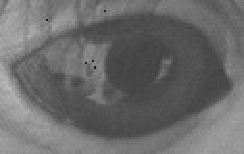
\includegraphics[width=0.3\textwidth]{figurer/monkbl01.pdf}}
  \makebox[0.45\textwidth][l]{
    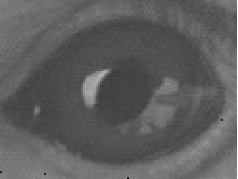
\includegraphics[width=0.3\textwidth]{figurer/monkbr01.pdf}}
  \hspace*{0.28\textwidth}(a)\hspace*{0.38\textwidth}(b)
  \paragraph{}
  \makebox[0.425\textwidth][r]{
    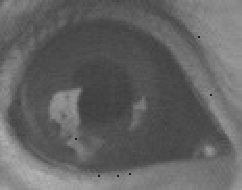
\includegraphics[width=0.3\textwidth]{figurer/monkbl02.pdf}}
  \makebox[0.45\textwidth][l]{
    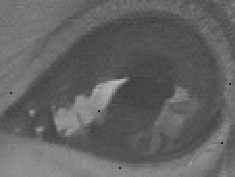
\includegraphics[width=0.3\textwidth]{figurer/monkbr02.pdf}}
  \hspace*{0.28\textwidth}(c)\hspace*{0.38\textwidth}(d)
  \paragraph{}
  \makebox[0.425\textwidth][r]{
    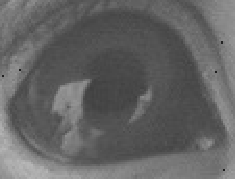
\includegraphics[width=0.3\textwidth]{figurer/monkbl05.pdf}}
  \makebox[0.45\textwidth][l]{
    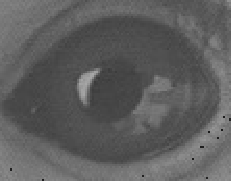
\includegraphics[width=0.3\textwidth]{figurer/monkbr03.pdf}}
  \hspace*{0.28\textwidth}(e)\hspace*{0.38\textwidth}(f)
  \caption{\label{fig:testimages}The test images used while developing
    and testing {\octopus}.}
\end{figure}

\noindent Throughout this chapter, a number of images of the monkey's
eye will be used to illustrate principles, examples and results.
These images, which constitute a subset of the images that were used
while developing and testing {\octopus}, are shown in
Fig.~\ref{fig:testimages}.  The image in Fig.~\ref{fig:compare}(a) is
identical to image (e) above.  The slight variation in size/resolution
of the images is due to the fact that they have been acquired by
manually clipping out of larger images the portion containing the eye,
as pointed out in the previous section.  Clearly, the image quality is
not very good.  Note in particular the strong reflections present in
the images, as well as their ``flat'' appearance.  Three factors
contribute to the bad quality:
\begin{description}
\item[Light conditions:] The images are from a non-IR video recording
  of the monkey, made under ``normal'' light conditions in the
  so-called {\em monkey laboratory\/}; that is, where the
  neurophysiological experiments of the Eckhorn-Bauer group take
  place.  ``Normal'' light conditions mean non-experimental; i.e., the
  light stems from ordinary fluorescent lamps in the ceiling of the
  laboratory.  The reflections in the images are of illuminated
  artifacts in the near surroundings of the monkey.  Note that in all
  images the reflections cover part of the pupil, thus making the
  pupil-contour non-elliptic.  Since reflections in an image are of a
  non-additive nature, and thus completely remove information about
  the regions they cover, they cannot be filtered out.
\item[The frame-grabber:] The ``flat'' appearance of the images is due
  to relatively low contrast.  This is a consequence of a bug in the
  frame-grabber, where increasing the contrast induces spurious dark
  pixels---``spots''---into the digitized frames.  The number of
  induced spots increases with the contrast.  Accordingly, a balance
  between high contrast and few induced spots had to be found.
  Actually, the induced spots have gray levels that are darker than
  the darkest gray level (15) in the ``uncorrupted'' image.  Note that
  a small number of spots are still present in the images.  Another
  factor which contributes to lowering the visual contrast is the fact
  that the darkest gray level in the images is not ``black'', but 15.
\item[Incorrect synch:] As can be seen, some of the images appear to
  be distorted along the vertical axis.  This applies particularly to
  image (e) and was caused by the synch of the frame-grabber not
  being calibrated to handle frozen frames, which were necessary in
  order to be able to control which frames were going to be digitized.
\end{description}

However, although the images can be characterized as bad, they are
good {\em test\/} images, apart from their low resolution, in that
their bad quality is apt to expose the weaknesses of the eye tracking
algorithm.  In the following, when referring to ``the given test
images'', the entire set of test images with which I have been working
is meant, not only those of Fig.~\ref{fig:testimages}.

\subsection{Structure of the Chapter}
\label{algot:intro:structure}

As was pointed out in the basic algorithm formulation in
Section~\ref{eval:approach:algo}, the algorithm decided upon can be
seen as consisting of two main steps: 
\begin{description}
\item[Step 1:] Apply a search strategy employing some sort of pixel
  filter to locate a point which unambiguously can be classified as a
  pupil point.
\item[Step 2:] Assign the pupil point returned by the search strategy
  to the origin of operation, and use line oriented edge detection on
  as high a number of line pairs as allowed by the time available in
  order to obtain as accurate an estimate of the centre position of
  the pupil as possible.
\end{description}

Section~\ref{algo:seek} presents the {\em swimming octopus\/} search
algorithm as a realization of the search strategy and pixel filter
required by Step 1, and Section~\ref{algo:pos} describes how Step 2 is
realized in {\octopus}; in particular, the gradient operators employed
are elaborated upon.  In Section~\ref{algo:eval}, {\octopus} is run on
the given test test images, and the results obtained are evaluated
with respect to accuracy and time consumption; and in
Section~\ref{algo:future}, the most important aspects pertaining to
the incorporation of {\octopus} in a complete eye-tracking system are
discussed.
